\section{High Energy Spectrum}
\begin{quotation}
	\raggedleft \it
	X-rays will prove to be a hoax! \\
	-- Lord Kelvin
\end{quotation}
It has already been shown that the fermion ball scenario can account for the cut-out in the IR while the black hole scenario in the
standard theory of accretion, cannot.
This is not, by far, the entire observed spectrum from Sgr A. Here we present some of the higher energy spectral data and briefly
discuss the problems and possible solutions for each of our 2 scenarios.

\subsection{X-Ray Spectrum}
Observations of Sgr A \cite{ref_baganoff} have revealed high emissions at X-ray wavelengths, coincident within 0.014 parsecs to the radio
source Sgr A*. This source corresponds to thermal bremsstrahlung emission with temperature $\sim 10^6$K, in agreement with \cite{ref_melia}.
Not only have these observations shown a distinctive quiescent state spectrum originating from the Sgr A* region,
but rapid `flaring' has also been observed. The X-ray luminosity increases by a
factor of 50 during this flaring state, Figure \ref{fig_fredxray} shows this flaring behaviour alongside the quiescent state.
This flaring suggests only one thing, a small compact object. Time variability measurements also suggest the emitting region not be larger
than 1.2 AU. An extended object such as the fermion ball cannot possibly create this sudden increase in luminosity.

\subsubsection{Iron Line or Fermion Decay}
\label{sec_fermiondecay}
There is, however, also a problem with the black hole scenario producing
such a spectrum. In the quiescent state, there is a peak at around 6.4keV. This peak is absent in the flaring state, and therefore suggests
that the flare `fuel' is of different composure. The peak itself corresponds to an emission line of iron K$_\alpha$, which would require a
gaseous temperature of $5\times 10^7$K. If we were to assume a black hole central object, then the only explanation would
be that any flaring is caused by comets, which are by nature water (and thus lacking the iron to produce the peak). This scenario is
statistically very unlikely, as we must be prepared to see flaring from all forms of fuel if the object is indeed a black hole.
\begin{figure}[ht]
	\begin{center}
	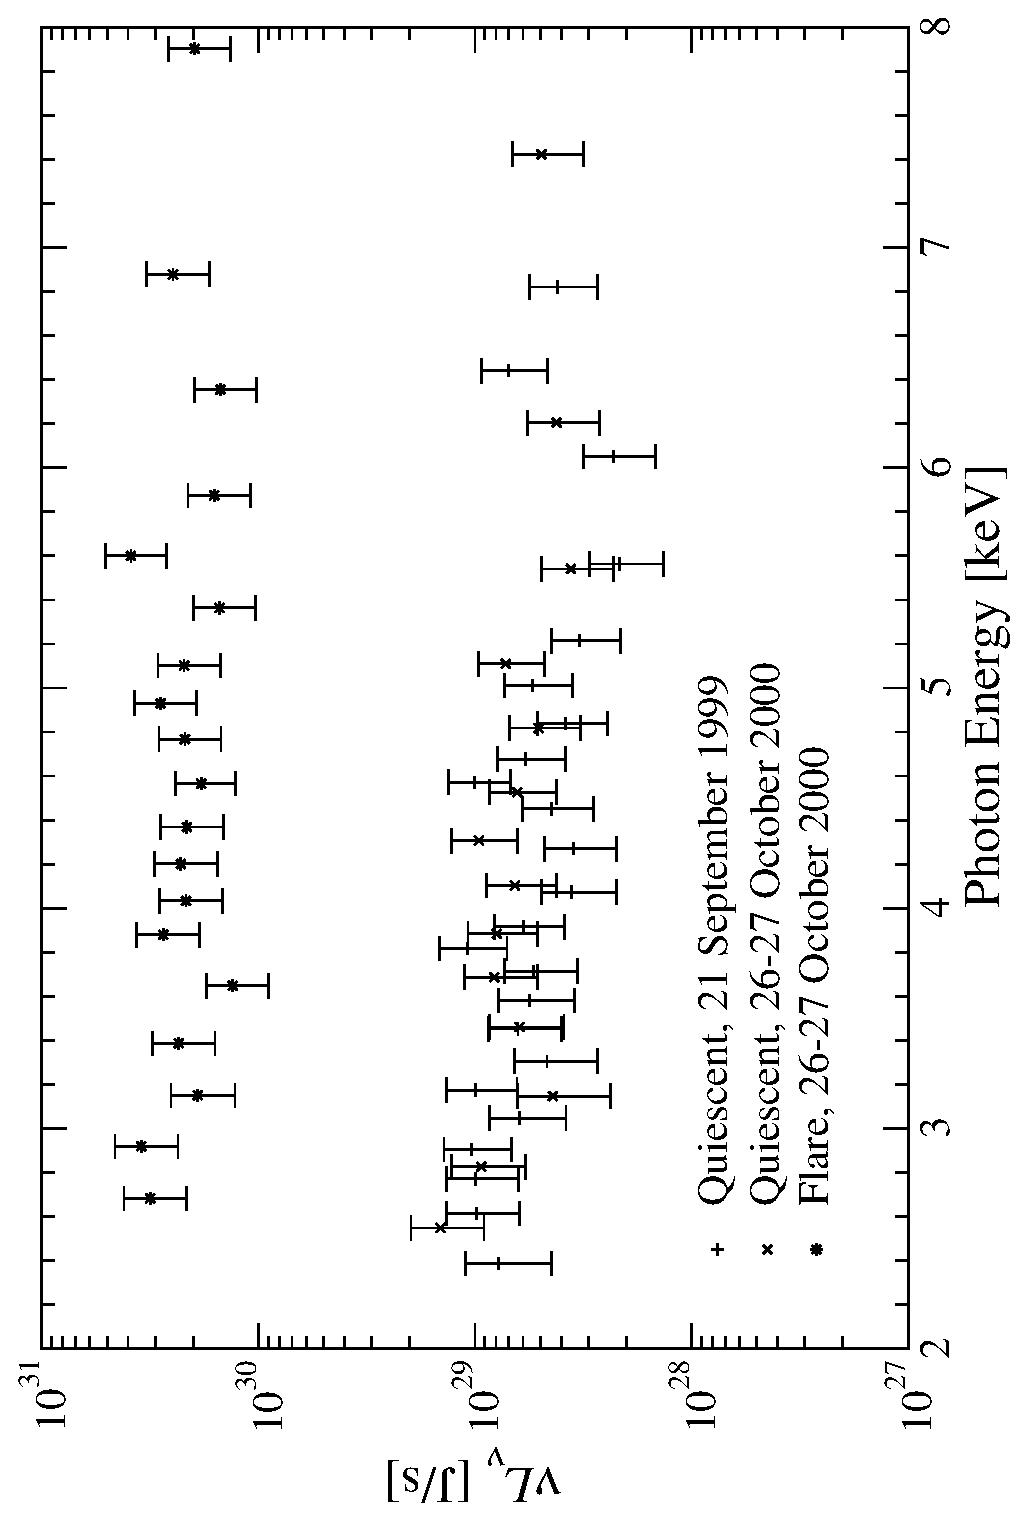
\includegraphics[angle=-90,width=0.9\textwidth]{eps/xray-nulum.eps}
	\caption{X-ray spectrum.}
	\label{fig_fredxray}
	\end{center}
\end{figure}

An alternative solution is to consider the possibility of another compact object in the vicinity of Sgr A*, such as an X-ray binary.
In the
black hole scenario, the binary would need to be between us and Sgr A*, and we would therefore eventually observe the source disappear around
the back of the black hole, but we are still left with the problem of the Fe K$_\alpha$ line. For the fermion ball scenario we place
the binary incident with Sgr A*, but we explain the 6.4keV peak by a completely different process altogether. As the fermion ball is by
nature, made of fermions, we expect them to decay. A Feynman diagram is shown for a possible decay path associated to a sterile neutrino which
results in a nearly massless active neutrino taking away half the energy.
\begin{figure}[!h]
	\begin{center}
	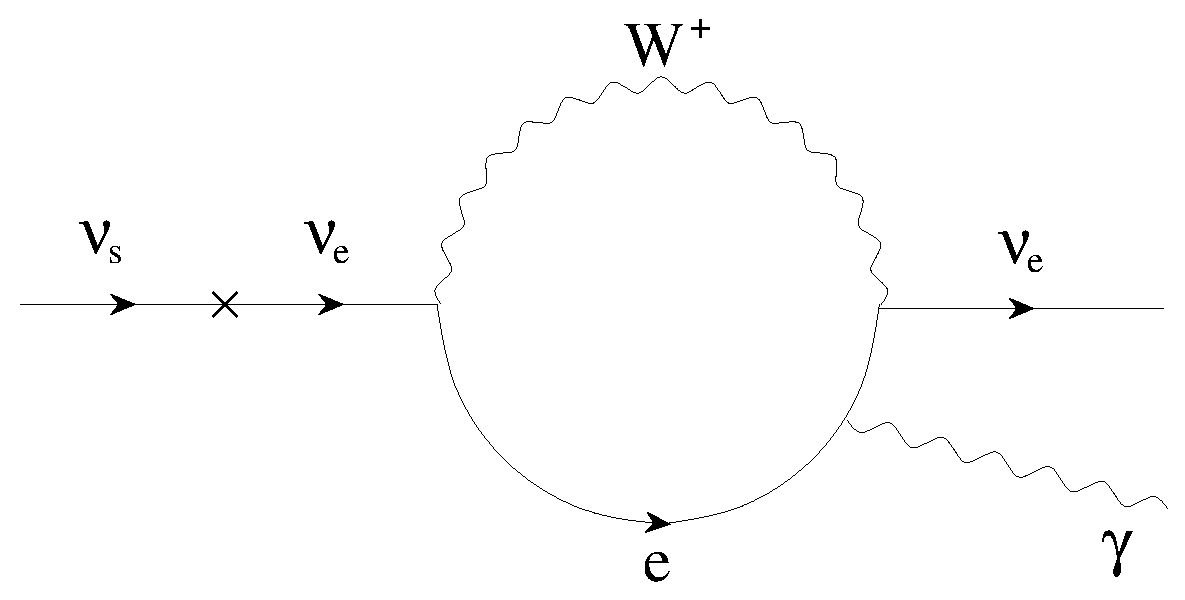
\includegraphics[angle=0,width=0.6\textwidth]{eps/fermiondecay.eps}
	\caption{Feynman diagram for the radiative decay of a sterile neutrino into an active neutrino
	and a photon of energy $\frac{m_{\nu_s}}{2}$.}
	\label{fig_feynmandiag}
	\end{center}
\end{figure}

\noindent
This photon with sharp energy should cause a peak in the spectrum which we may
observe. If we were to speculate that the 6.4keV peak was evidence of this process, we would require a fermion ball containing fermions of
mass 12.8keV. This is obviously too low a value to be consistent with Section \ref{sec_fermionlimits}. However, if the fermions were of the
degeneracy 4 variety, then we would be able to use Equation (\ref{eqn_classicalfermiondegeneracyrelation}) to say that the fermion ball would
display the same mass distribution with $g$=4, $m_\nu$=12.8keV as with $g$=2, $m_\nu$=15.2keV. We have already shown that 16keV
fermions display properties capable of explaining orbital motion of cluster stars and the IR cut-out, it is also quite possible to
show the same for 15.2keV fermions. Considering errors in the peak measurement, fermions of up to $g$=4, $m_\nu$=13.5keV,
equivalent to $g$=2, $m_\nu$=16keV would also produce such a spectral line.

Another advantage of the X-ray binary presence is that we would have a possible source for the synchrotron emission which explains the
radio and microwave spectrum, missing from the accretion model.

However, due to the constant influx of fast moving stars through the galactic centre, we should expect an X-ray binary resident
at the centre to be ejected after a short period of time. This X-ray binary phenomenon could therefore be a short term effect.

\subsubsection{On Possible Measurement of $z$ and $v_z$ for Nearby Stars}
\label{sec_zandvz}
The photons from the X-ray flare will be incident upon stars near the galactic centre, including S0-1, S0-2 and S0-4. As the
resolution of X-ray maps is not enough to see a reflection from these stars directly, we may look at the IR spectra
and possibly observe corresponding activity, initiated by the X-ray flare. By measuring the time delay between the X-ray
flare (assumed to be from Sgr A*) and IR activity at a neighbouring star, we may calculate $z$ for that star.

It may also be that such a flare would intensify well known spectral lines, allowing for a corresponding measurement of $v_z$.
Such a measurement would instantly discern between black hole or extended source models of the galactic centre, by
using the phase space analysis presented in Section \ref{sec_futureps}.
We now show how such a time delay measurement would lead to a value of $z$, Figure \ref{fig_geomfindzvz}.
\begin{figure}[!h]
	\begin{center}
	\includegraphics[angle=0,width=0.7\textwidth]{eps/zmeasure.eps}
	\caption{Geometry of the photons from the X-ray flare and response.}
	\label{fig_geomfindzvz}
	\end{center}
\end{figure}

\noindent
We measure $\Delta t=t_{{\rm {\it response}}}-t_{{\rm {\it flare}}}$. The distances $F$ and $I$ in terms of the incident times are
$F=ct_{{\rm {\it flare}}}$ and $I+R=ct_{{\rm {\it response}}}$ where $c$ is the speed of light. It is clear that $I=F-z$, giving us
a suitable form of equations which we may solve for $z$, giving
\begin{equation}
	z=\frac{\left(x^2+y^2\right)}{2c\Delta t} -\frac{c\Delta t}{2}
\end{equation}

\subsection{$\gamma$-Ray Spectrum}
Although it has been mentioned that there is a $\gamma$-ray spectrum associated with the galactic centre \cite{ref_gamma}, it is however
only spatially resolved to within a radius of 0.2 degrees from Sgr A*. Since we are dealing with objects already constrained within 0.5
arcsec, the $\gamma$-ray spectrum cannot conclusively be associated with Sgr A*, except as an upper limit.
